\documentclass[10pt,letterpaper]{article}

\usepackage[usenames, dvipsnames]{color}
\usepackage{hyperref}
\hypersetup{
    colorlinks = true,
    citecolor = {black},
    % linkcolor = {WildStrawberry},
    % urlcolor = {WildStrawberry}
    linkcolor = {black},
    urlcolor = {black}
}
\usepackage{breakurl}
\usepackage{cogsci}
\usepackage{pslatex}
\usepackage{apacite}
\usepackage{graphicx}
\usepackage{caption}
\usepackage{subcaption}
\usepackage{amsfonts}
\usepackage{amsmath}

\newcommand{\w}[1]{\emph{#1}}
\newcommand{\todo}[1]{{\color{red}#1}}
\newcommand{\ndg}[1]{{\color{green}#1}}

\title{Extremely costly intensifiers are stronger than quite costly ones}
 
\author{{\large \bf Erin D.~Bennett} (erindb@stanford.edu), {\large \bf Noah D.~Goodman} (ngoodman@stanford.edu)\\
  Department of Psychology, Stanford University.}
  
\begin{document}

\maketitle

\begin{abstract}

We show that the wide range in strengths of intensifying degree adverbs (e.g.~\w{very} and \w{extremely}) can be partly explained by pragmatic inference based on differing cost, rather than differing semantics.
The pragmatic theory predicts a linear relationship between the meaning of intensifiers and their length and log-frequency.
We first test this prediction in three studies, using two different dependent measures, finding that higher utterance cost (i.e. higher word length or surprisal) does predict stronger meanings.
In two additional studies we confirm that the relationship between length and meaning is present even for novel words.
We discuss the implications for adverbial meaning and the more general question of how extensive non-arbitrary form-meaning association may be in language.

\textbf{Keywords:} 
intensifiers; degree adverbs; scalar adjectives; pragmatics; m-implicature
\end{abstract}

\section{Introduction}

How do different words get their meanings?
For instance, why is an ``extremely good paper'' better than a ``quite good paper''?
The traditional answer \cite{de_saussure_nature_1916} is that different meanings have been arbitrarily and conventionally assigned to the different word forms.
This view has been challenged by a number of examples in which word meaning appears to be non-arbitrarily related to properties of the word.
In some cases, the phonetic form of a word is systematically related to its meaning, for example rounded vowels and voiced consonants tend to refer to round objects \cite{kohler_gestalt_1970, ramachandran_synaesthesiawindow_2001, holland_physiognomic_1964, davis_fitness_1961}.
In other cases, orthographic form is diagnostic of meaning, for example, speakers of Hebrew who have never seen Chinese characters are nonetheless above chance at matching them to their corresponding Hebrew words \cite{koriat_figural_1979}.
Similarly, the length of words predicts aspects of their meanings: across languages longer words refer to more complex meanings \cite{lewis_conceptual_2016}.
Open questions remain about the systematic factors that can influence meaning and the source of these effects.

In this paper, we explore adjectival intensifiers\footnote{
Intensifiers are adverbs that modify scalar adjectives so that the interpretation of the intensified adjective phrase is more extreme than the interpretation of the bare adjective phrase.
The word ``intensifier'' is often used to denote the full range of degree adverbs, be they ``amplifiers'', or ``downtoners'' \cite{quirk}.
The ``intensifiers'' we are looking at in this paper are, according to this typology, ``amplifiers'' because they increase (rather than decrease) the threshold associated with a gradable predicate.
This typology also distinguishes between two different kinds of amplifiers: those that increase an adjective maximally (e.g. \w{completely} and \w{utterly}) and those that merely increase (e.g. \w{greatly} and \w{terribly}).
We do not make this distinction.
The word ``intensifier'' is sometimes used for a completely different linguistic phenomenon, where a reflexive is used for emphasis, e.g. ``The king himself gave the command,'' which we do not analyze in this paper. 
},
like \w{extremely} and \w{quite}, as a case study in which to empirically explore the relationship of meaning to factors like word form and distribution of usage.
Intensifiers form a good case study because they are amenable to simple quantitative measures of meaning: Many adjectives correspond to concrete numeric scales, and intensifier's strength can be measured as the numeric extent to which it shifts the interpretation of such a scalar adjective. They are of interest because theoretical considerations, which we lay out below, suggest a relationship between intensifier meaning and their communicative cost (i.e. frequency and length).
This account of intensifier meaning adds to a growing body of literature exploring how principles of recursive, rational communication shape language interpretation \cite[e.g.]{grice_logic_1975, frank_predicting_2012, goodman_knowledge_2013, franke_quantity_2011, russell_probabilistic_2012, kao_nonliteral_2014, bergen_pragmatic_2014}.

In the next \hyperref[sec:semantics]{section}, we discuss a minimal semantics for intensifiers, building off of previous work on scalar adjectives and formalized concretely in our \hyperref[app:model]{Appendix}.
We show how pragmatic effects predict systematic variation in the meanings of intensifiers: the meanings of intensifiers are expected to be influenced by their form (in length) and their distribution (frequency) of usage.
The impact of word length is reminiscent of the results of \citeA{lewis_conceptual_2016}, who studied noun categories.
While word frequency is known to have major effects on sentence processing \cite[e.g.]{levy_expectation-based_2008}, the prediction that frequency should affect meaning is more surprising.

We confirm, in our first series of studies (Studies \hyperref[sec:study1a]{1a}, \hyperref[sec:study1b]{1b}, and \hyperref[sec:study2]{2}), that English intensifiers in adjective phrases are indeed interpreted as much stronger for both longer and less frequent intensifiers.
This holds in quantitative judgments of meaning and in forced comparisons, and across a number of adjectival dimensions.
In our second set of studies (Studies \hyperref[sec:study3]{3} and \hyperref[sec:study4]{4}), we replicate this finding, and extend it to novel intensifiers, showing that length is a significant predictor of the strength of an intensifier’s meaning even in the absence of any conventional meaning.
We conclude with a discussion of different interpretations of these phenomena and future directions.

\section{The semantics of intensifying degree adverbs \label{sec:semantics}}

Our paper focuses on intensifying degree adverbs applied to scalar adjectives.\footnote{
  Some of these intensifiers can also apply to verbal and nominal predicates, and different restrictions apply for different intensifiers, e.g. \w{I truly like carrots} is an acceptable utterance, whereas \w{I very like carrots} is not. See \citeA{bolinger_degree_1972} for a discussion.
 }
Scalar adjectives have been described as having a threshold semantics \cite{kennedy_vagueness_2007}, where, for example, \w{expensive} means ``having a price greater than $\theta$'' and $\theta$ is a semantic variable inferred from context (e.g., \$100).
Above the threshold degree $\theta$, the adjective is true of an object, and below, the adjective is false.
\citeA{lassiter_context_2013} build on the Rational Speech Acts (RSA) framework \cite{frank_predicting_2012, goodman_knowledge_2013} to give a formal, probabilistic model of how this threshold might be established by pragmatic inference that takes into account statistical background knowledge (such as the distribution of prices for objects).
We return to this model below and present a full model in the \hyperref[app:model]{Appendix}.

Previous researchers have proposed that adjective phrases modified by intensifiers have the same semantics as unmodified adjective phrases, except with new, higher thresholds \cite{kennedy_scale_2005, klein_semantics_1980, wheeler_attributives_1972}.
That is, some threshold, inferred from context, exists above which objects are \w{expensive} and below which they are not, and the intensifier \w{very} determines a new, higher threshold for the adjective phrase \w{very expensive}.
These researchers suggest that the intensified thresholds are determined by first collecting the set of objects in the comparison class for which the bare adjective is true, and then using that as the comparison class to infer a new threshold, i.e. \w{very expensive laptop} means ``expensive for an expensive laptop''.
This analysis results in the expected intensification of adjectives (``expensive for an expensive laptop'' has a higher threshold for being true than simply ``expensive for a laptop'') and is appropriately sensitive to different domains (e.g. the absolute difference in price between thresholds for \w{expensive} and \w{very expensive} is much higher in the context of ``That space station is very expensive,'' than in the context of ``That coffee is very expensive.'').
However, this proposal does not distinguish between the graded strengths of different intensifiers, for example, \w{very expensive} and \w{phenomenally expensive}.

Intuition suggests that different intensifiers do have different strengths (e.g. \w{outrageously} seems stronger than \w{quite}), and we provide further evidence of this in our studies, where participants interpret and compare different intensifiers.
It could be that the degree of strength of different intensifiers is conventionally specified by the lexicon. But the semantics must then specify how these entries affect the very flexible threshold of the relevant adjective.
In addition, the multitude of intensifiers \cite{bolinger_degree_1972} and their apparent productivity\footnote{For example, \w{altitidinously expensive} is not in common usage, but one can easily interpret \w{altitidinously} as a novel intensifier.}
suggest a more parsimonious solution would be welcome. 
That is, having a lexically determined meaning for each different intensifier might overlook the similarity among words of this class.
In the account that follows, we build minimally on existing models of adjective interpretation and rational communication to articulate a model of intensified adjective phrase interpretation.

\subsection{Intensification as an M-implicature}

We explore the idea that an adjective phrase with an intensifying degree adverb derives much of its meaning from a M(arkedness)-implicature \cite{levinson_presumptive_2000}: more marked (costly to utter) versions of an adjective phrase will be interpreted as implicating higher values (e.g. in case of the adjective \w{expensive}, higher prices). 
Given two possible utterances a speaker could say to communicate the same meaning, a speaker will usually choose the less costly utterance.
If the speaker instead chooses a more costly utterance (e.g. ``I got the car to start'' as opposed to ``I started the car''), they may be doing so in order to communicate something more distinct, intense, or unusual (e.g. ``I got the car to start, but it was unusually difficult'').
In other words, the marked form corresponds to the marked meaning.
If scalar adjectives include a free threshold variable inferred from context, then the speaker's use of a longer, intensified adjective phrase could lead the listener to infer that the threshold for this adjective phrase is unusually extreme relative to other, less costly phrases that the speaker could have used. 

To realize such an M-implicature, we suggest extending \citeA{lassiter_context_2013}'s probabilistic model of scalar adjective interpretation slightly.
% by assigning a separate threshold to each intensified (or bare) adjective phrase.
We assume that each time a scalar adjective is used, in each phrase, it introduces a free threshold variable---a new token threshold is inferred for each access of the lexical entry of the adjective.
The set of thresholds, for the actual sentence and all alternative sentences, is then established by a pragmatic inference that takes into account the differing costs of the sentences.
The intensifiers themselves do not contribute to the semantics but increase the cost of the utterance, thus affecting pragmatic inferences.
This model is described in detail in the \hyperref[app:model]{Appendix}.
As in previous RSA models that include utterances with similar semantics but different costs \cite{bergen_thats_2012, bergen_pragmatic_2014}, we find an M-implicature, such that more costly intensifiers result in stronger adjective phrases.
As illustrated in the \hyperref[app:model]{Appendix} this relationship is expected to be approximately linear, resulting in a straightforward quantitative hypothesis that we evaluate against empirical data in our studies.

We view this model as an illustrative caricature of intensifier meaning: In this model intensifiers contribute \emph{nothing} to the literal, compositional semantics.
Yet, pragmatic interpretation yields a spectrum of effective meanings for the intensifiers, determined by their relative usage costs.
This predicts an empirically testable systematic variation in meaning as a function of cost.
It is very likely that the meaning of individual intensifiers includes idiosyncratic, conventional aspects in addition to these systematic factors.
This would be expected to show up as residual variation not predicted by cost, but would not nullify the hypothesized relationship between cost and meaning.
This account applies straightforwardly only to intensifying degree adverbs; ``de-intensifying'' adverbs that effectively lower the threshold will require further work to explain.

%This implies that different adjectival phrases (e.g.~``very expensive watch'' and ``extremely expensive watch'') have equivalent meanings, though with thresholds that will be separately assigned based on context.
% Further we propose that intensifiers contribute \emph{nothing} to the literal, compositional semantics\footnote{We take this strong view for rhetorical purposes. It is highly likely that some intensifiers have other aspects of meaning.}. 
%  \emph{However}, the intensifiers do affect the production cost of the corresponding sentences, and it is this cost difference that results in meaning differences.

% 


\subsection{Factors affecting utterance cost}

We have identified an intensifier's cost as a potentially critical determiner of its interpreted meaning.
To connect this prediction to empirical facts, we still must specify (at least a subset of) the factors we expect to impact cost.
The most natural notion of cost is the effort a speaker incurs to produce an utterance. 
his could include cognitive effort to access lexical items from memory, articulatory effort to produce  the sound forms, and other such direct costs.
Speakers might also seek to minimize comprehension cost for their listeners, resulting in other contributions to cost. 
For the purposes of this paper, we restrict ourselves to the most obvious contributors to production cost and use proxies that are straightforward to quantify: length (longer utterances are more costly)\footnote{
  We measure length in number of syllables, although length in characters (which might be a more relevant source of utterance cost in a written format) has similar predictive power to syllable length in all of our analyses.
}
and frequency (rarer intensifiers are harder to retrieve from memory in production and therefore more costly).
In a number of different tasks, lexical frequency affects difficulty in an approximately logarithmic way.
For instance, word recognition time \cite{mccusker_determinants_1977} and reading time in context \cite{smith_effect_2013} are both logarithmic in frequency.
We thus use the log-frequency (whose negative is also called \emph{surprisal}) as the quantitative contribution to cost.

Our model predicts a linear contribution of longer and higher surprisal intensifiers to the meaning of an adjectival phrase (see the \hyperref[app:model]{Appendix} for more detail). 
This leaves open the the relative importance of length and surprisal (as well as other factors that might enter into cost), which can be explored via regression models.

\section{Utterance cost predicts intensifier strength}

The proposal detailed above predicts an association between measures of cost and strength of interpretations.
In our first series of studies, detailed in this section, we tested whether our measures of communicative cost can in fact predict intensifier strength.

We used two measures of intensifier strength.
Our first measure of intensifier strength (used in Studies \hyperref[sec:study1a]{1a} and \hyperref[sec:study1b]{1b}) was asking participants for a numeric interpretation of intensified adjective phrases.
Our second measure (used in Study \hyperref[sec:study2]{2}) was asking participants to rank the strength of adjective phrases that differed only in their intensifier.
The first measure allowed us to compare our full set of intensifiers to one another on a numeric scale.
The second allowed us to test our hypothesis on a wider range of adjectives at once, some of which (e.g. \w{beautiful}) correspond to more abstract, non-numeric scales.

\subsection{Study 1a \label{sec:study1a}}

In Study \hyperref[sec:study1a]{1a}, we tested the qualitative prediction that as the communicative cost of an intensifier increases, so will the numeric interpretation of the adjective phrase it is part of.
We tested this prediction by eliciting free-response price estimates from participants for phrases such as \w{very expensive watch} and determining whether the prices participants responded with were correlated with a independent measures of communicative cost.

\subsubsection{Methods}

\paragraph{Participants}

30 participants with US IP addresses were recruited through Amazon’s Mechanical Turk and paid \$0.40 for their participation. 1 participant was excluded from the analysis for admitting that they did not think they followed the instructions in a post-experiment survey and another for not being a native speaker of English.

\paragraph{Items}

The sentences in the study included intensifiers paired with the adjective \w{expensive} (Figure \ref{fig:question_study1a}).
There were three categories of objects (\w{laptop}, \w{watch}, and \w{coffee maker}) and 40 intensifiers (see Table \ref{table:intensifiers_study1a}).

The intensifiers in our study were collected from word lists online and searching thesauri for more intensifiers.
We chose intensifiers that have a wide range of frequencies and excluded intensifiers that are either more commonly used to signal affect than to signal degree (e.g. \w{depressingly expensive} might indicate a degree, but it mainly indicates affect) or are ambiguous between other parts of speech (e.g. \w{super} can be used as an intensifier, as in ``super expensive'', but it can also be used as an exclamation, as in ``Super!'').

We chose the domain of price for Study \hyperref[sec:study1a]{1a} and used only the adjective \w{expensive}.
Because price constitutes a quantitative scale with standard units (dollars for our US participants), this allowed us to quantitatively measure the relative strengths of different intensifiers.

\paragraph{Procedure\footnote{A demo of Study \hyperref[sec:study1a]{1a} can be found at \url{http://cocolab.stanford.edu/links_for_papers/bennett2017extremely/experiments/Study1a/.}}}

We asked participants to estimate the prices of different objects based on different descriptions of those objects. 

Each participant gave price judgments for every intensifier-category pairing in a randomized order (different for different participants), for a total of 120 price judgments per participant.  

The only allowable characters in responses were the digits 0-9 and (optionally) one decimal point (.) followed by two digits. All other responses were immediately rejected.
Participants were prevented from continuing until they provided a valid numeric response for each trial.

\begin{figure}[ht]
\begin{center}
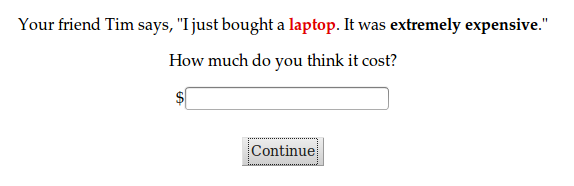
\includegraphics[width=0.4\textwidth]{exp1-q.png}
\end{center}
\caption{Screenshot from Study \hyperref[sec:study1a]{1a} target question.} 
\label{fig:question_study1a}
\end{figure}

\begin{table}[ht]
 \begin{center}
 \footnotesize
  \caption{Intensifiers from Study \hyperref[sec:study1a]{1a}, number of occurences in Google Web 1T 5grams corpus, and length in syllables.}
  \label{table:intensifiers_study1a}
  \begin{tabular}{llc}
   \hline
   ngram & frequency & length \\
    \hline
    surpassingly & 11156 & 4 \\
    colossally & 11167 & 4 \\
    terrifically & 62292 & 4 \\
    frightfully & 65389 & 3 \\
    astoundingly & 73041 & 4 \\
    phenomenally & 120769 & 5 \\
    uncommonly & 135747 & 4 \\
    outrageously & 240010 & 4 \\
    fantastically & 250989 & 4 \\
    mightily & 252135 & 3 \\
    supremely & 296134 & 3 \\
    insanely & 359644 & 3 \\
    strikingly & 480417 & 3 \\
    acutely & 493931 & 3 \\
    awfully & 651519 & 3 \\
    decidedly & 817806 & 4 \\
    excessively & 877280 & 4 \\
    extraordinarily & 900456 & 6 \\
    exceedingly & 977435 & 4 \\
    intensely & 1084765 & 3 \\
    markedly & 1213704 & 3 \\
    amazingly & 1384225 & 4 \\
    radically & 1414254 & 3 \\
    unusually & 1583939 & 4 \\
    remarkably & 1902493 & 4 \\
    terribly & 1906059 & 3 \\
    exceptionally & 2054231 & 5 \\
    desperately & 2139968 & 3 \\
    utterly & 2507480 & 3 \\
    notably & 3141835 & 3 \\
    incredibly & 4416030 & 4 \\
    seriously & 12570333 & 4 \\
    truly & 19778608 & 2 \\
    significantly & 19939125 & 5 \\
    totally & 20950052 & 3 \\
    extremely & 21862963 & 3 \\
    particularly & 41066217 & 5 \\
    quite & 55269390 & 1 \\
    especially & 55397873 & 4 \\
    very & 292897993 & 2
  \end{tabular}
 \end{center}
\end{table}

\subsubsection{Corpus Methods}

Table~\ref{table:intensifiers_study1a} shows word frequency and length in syllables for the intensifiers used in Study \hyperref[sec:study1a]{1a}.
The frequencies were collected from the Google Web 1T 5-grams database \cite{brants_web_2006}.\footnote{
  We also ran the same analyses on frequency information collected from the Google Books American Ngrams Corpus \cite{michel_quantitative_2011} and found similar results.
}
In the analysis below we use word length and word surprisal (negative log-frequency) as proxies for a word's cost, as motivated above.
The syllable lengths of our intensifiers and the surprisals were correlated ($r = 0.26$).
This correlation makes it somewhat difficult to determine the effect of one measure of cost above and beyond the other.
In our first series of studies, we focus on the primary effect of surprisal, since we have more range in surprisal across intensifiers than in length and since we manipulate length in syllbles for our next series of studies.
However, we model both measures of communicative cost in our analyses: we include both predictors in regressions and report likelihood-ratio tests between the full model and simpler models.

\subsubsection{Analysis}

Prices that participants give obviously vary systematically with the object (expensive laptops tend to be more expensive than expensive coffee makers).
Prices are also likely sensitive to variation across participants due to their different beliefs about likely prices.
Because we have few objects, we are unable to model the variation due to object, but because we have many intensifiers (they are fully crossed with objects), normalizing is fairly effective at converting all objects to the same scale.
We are not theoretically interested in the variation due to objects, and so in order to compare intensifiers across these objects, we first normalized log-transformed prices within participant and object.
We used the logarithm of participants' price estimates because of evidence that people's representation of numbers, including prices, is logarithmic \cite{fechner_elements_1860}.\footnote{
  I.e. the perceptual distance between two prices the same dollar amount apart is more for small numbers (e.g. \$3 and \$6) and less for large numbers (e.g. \$1,543 and \$1,546).
}

We ran a linear mixed effects regression to predict scaled price estimates. We included centered fixed effects of length and surprisal. To model random effects due to participant, we only included random slopes, since the normalization gives each participant an intercept of 0.  We also included a random intercept for intensifier to model any idiosyncratic meaning there might be to a particular intensifier beyond communicative cost. 
The predicted mean $y_{ij}$ for the $i^{th}$ intensifier and the $j^{th}$ participant under this model is shown in Equation \ref{eq:study1}, where $f_i$ represents the surprisal of the $i^{th}$ intensifier and $l_i$ represents its length. %with random by-intensifier intercepts $I_i$ and random by-participant slopes $P_{1j}$ and $P_{2j}$.


\begin{equation}
\label{eq:study1}
y_{ij} = \beta_0 + {U_0}_{i} + ({U_1}_{j} + \beta_1) {f}_{i} + ({U_2}_{j} + \beta_2) {l}_{i}
\end{equation}

As previously noted, surprisal and length in syllables are correlated in this set of intensifiers (r=0.26). We focus on surprisal as our primary effect, but we are also interested in the independent contribution of length in syllables. We focus on surprisal as our primary effect, but we are also interested in the independent contribution of length in syllables. To address the independent effects of these variables, we ran model comparisons using log likelihood, leaving out information about one of the predictors. We also ran two additional mixed effects reggressions: one in which the suprisal is first residualized against syllables (using ordinary linear regression), and one where syllables is residualized against surprisal.

\subsubsection{Results}

If the meaning of an intensifier is stronger for higher cost intensifiers, we would expect to find that as surprisal increases and length in syllables increases, the prices participants give will also increase. 
We find that this is the case for surprisal, but do not show a significant effect of syllable length beyond the effect of surprisal.
Our results are shown in Figure~\ref{fig:plot_study1a}, in a way that highlights the surprisal predictor. 

%The full regression shown in Equation was significant ($F(,)=__.__,p<0.___$), with an $R^2$ of $0.___$.
We found a significant effect of surprisal ($b=0.106,t(38.9)=3.411,p=0.0015$) such that less frequent words tend to be associated with higher price estimates.
In this regression, we did not a significant effect of syllable length ($b=0.133,t(39.9)=1.717,p=0.0936$), above and beyond surprisal.
%We also found a significant effect of syllable length ($b=0.133, t(27)=5.823, p<0.0005$), above and beyond surprisal.

Because surprisal and syllable-length are correlated, in addition to the analysis reported here we also used likelihood ratio tests to compare the full model to models with only one of the two predictors.
These tests show that length in syllables alone account for the data less well than the full model ($\chi^2(8)=17.055, p<0.0005$) and that surprisal alone also accounts for the data less well than the full model ($\chi^2(8)=13.697, p<0.0005$), suggesting that both might separately contribute to the cost of the utterance.
When length was residualized with respect to suprisal, both the residuals ($b=0.106,t(38.9)=3.411,p=0.002$) and length ($b=0.202,t(40.9)=2.693,p=0.010$) were significant predictors of scaled ratings. However, when surprisal was residualized with respect to length, surprisal ($b=0.12, t(39.9)=3.985, p<0.0005$) but not the residuals ($b=0.133,t(39.9)=1.717,p=0.0936$) was a significant predictor of scaled ratings. This discrepency is likely a due to the fact that, since length in syllables is a discrete value taking one of 6 values, whereas surprisal is continuous, length can be more informatively predicted from surprisal (different surprisals can map onto approximately the same length) than surprisal can be predicted from length (the same length cannot map onto different surprisals).
%This suggests that both surprisal and length in syllables may independently contribute to the strength of an intensifier.
%computed length-corrected surprisals by regressing the raw surprisals onto word length in syllables using linear regression with a single main effect of word length. The residuals of this model, length-corrected surprisals, were used for the surprisal predictor in similar analyses to the ones we report, and we consistently found similar results. This suggests more strongly that surprisal and syllable length \emph{both} independently contribute to participants' estimates.
%\ndg{doesn't this mean that we do need length in addition to surprisal, thus confirming the length prediction?}
% yeahhh....

Overall, we confirmed our main prediction that intensifiers that are less frequent (and therefore are more costly to communicate) also tend to be interpreted as having stronger meanings, at least when used to modify the adjective \emph{expensive}.
We found inconclusive results for our secondary prediction that length (another factor in communicative cost) has any effect beyond that of surprisal.
This ambiguity motivated a more sensitive dependent measure in Studies 2 and 4.
%Furthermore, the relationship appears to be linear in surprisal and length, as predicted by the M-implicature proposal introduced above.

\begin{figure}[ht]
\begin{center}
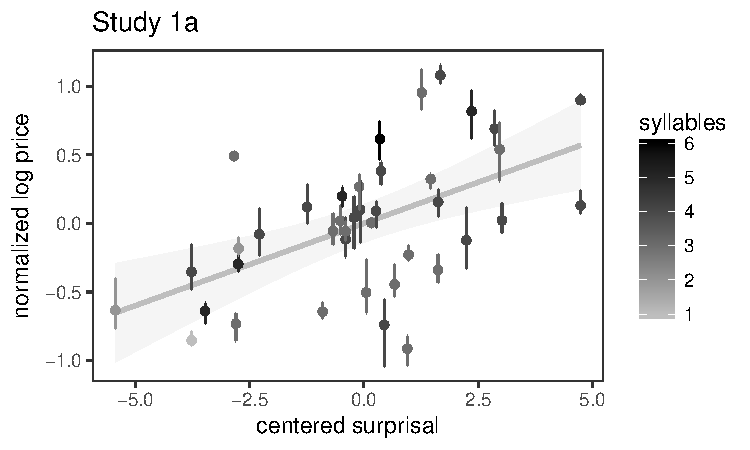
\includegraphics[width=0.5\textwidth]{images/plot_study1a.pdf}
\end{center}
\caption{Results of Study \hyperref[sec:study1a]{1a}. As surprisal and length in syllables increase, participants' scaled free response prices increase.} 
\label{fig:plot_study1a}
\end{figure}

\subsection{Study 1b \label{sec:study1b}}

Our initial selection of intensifiers was somewhat haphazard, being chosen partly to give the best (intuitive) chance of observing an effect. 
To show that there was no implicit bias induced by this selection, we next replicated using a revised, and more systematic, set of intensifiers.
We additionally took this opportunity to increase the sample size, guided by a power analysis based on the results of \hyperref[sec:study1a]{1a}.

\subsubsection{Methods}

\paragraph{Participants}

We wanted enough participants for a power level of 0.8 for the principal effect of surprisal.
Power analyses for mixed effects models with continuous predictors are not analytically straightforward, and so we approximated the number of participants necessary for our desired power by bootstrapping.
We used the data from our original Study \hyperref[sec:study1a]{1a} to simulate alternative possible datasets with different numbers of intensifiers and participants.
For each of 100 iterations, we sampled with replacement from Study \hyperref[sec:study1a]{1a} a set of $P$ participants and a set of $I$ intensifiers, varying $P$ and $I$.
We created a resampled dataset where we crossed the resampled participants with the resampled intensifiers and collected the corresponding responses for each pair.
For each resampled dataset, we ran the regression model from Study \hyperref[sec:study1a]{1a}.
We computed the proportion of runs in which the surprisal term was significant and interpreted this as the power of such a study.

We found that our original Study \hyperref[sec:study1a]{1a} was somewhat underpowered by this metric (statistical power was near 0.70 for the surprisal regressor, our principal effect of interest).
For the replication, we determined that with the 71 intensifiers we collected from grammars of English (described below), 50 was the minimum number of subjects for power at the 0.8 level for the surprisal term.
We doubled this amount for a goal of 100 participants for the replication.
(Despite having sufficient power for the surprisal term, our bootstrapped power analysis suggests that even with 100 participants, the power for the length term in the model is only 0.29. We address this instead, with a direct manipulation of length, in experiments 4 and 5.)
Due to a slight error in data collection, we actually recruited 108 participants.

Following this power analysis, 108 participants with US IP addresses were recruited through Amazon’s Mechanical Turk and paid \$1.00 for their participation. 1 participant was excluded from the analysis for admitting that they did not think they followed the instructions in a post-experiment survey and another for not being a native speaker of English.

\paragraph{Items}

For Study \hyperref[sec:study1b]{1b}, we again used \w{expensive} as the adjective for the intensifiers to modify, and we again collected responses as prices in dollars.
We used the same objects (\w{laptop}, \w{watch}, and \w{coffee maker}) as in Study  \hyperref[sec:study1a]{1a}.

In Study  \hyperref[sec:study1a]{1a} and the remaining studies detailed in this paper, our choice of the set of intensifiers to include was somewhat arbitrary and collected after formation of our hypothesis.
To address the concern that this might bias our results, we followed a more systematic procedure for generating a list of intensifiers for our replication Study \hyperref[sec:study1b]{1b}.
We sought out English grammars that listed intensifiers.
Since no single source contained the number of intensifiers desired for sufficient power in Study \hyperref[sec:study1b]{1b}, our process for collecting intensifiers in this replication was to combine word lists from multiple grammars of English.
We first found 12 grammars of English that mentioned one of the following terms: ``intensifiers'', ``adverbs of degree'', or ``amplifiers'' \cite{aarts_oxford_2014,douglas_longman_2000,declerck_comprehensive_1991,garner_chicago_2016,givon_english_1993,greenbaum_oxford_1996,huddleston_cambridge_2002,huddleston_introduction_1984,nelson_english:_2010,quirk_grammar_1972,quirk_students_1990,van_gelderen_introduction_2010}.
Most of these grammars mentioned examples of such words, and many contained lists of them.
The average length of such a list or collection was approximately 21 words.
We collected an aggregate list of all words that occurred in an ``intensifiers'', ``adverbs of degree'' or ``amplifiers'' list in at least one grammar.
Some ``downtoners''/``diminishers'' were mixed into some of these lists (e.g. \w{slightly}, \w{barely}).
Some other intensifiers cannot occur felicitously as simple pre-modifiers (e.g. \w{a lot}, \w{indeed}) and therefore would not fit in the same syntactic frame as the other intensifiers.
Other intensifiers were marked as occurring exclusively in British English (e.g. \w{bloody}, \w{jolly}), and since our participants were restricted to US IP addresses, we did not think these words would be as appropriate to include.
In addition, some lists included comparative degree adverbs like \w{more}.
We excluded downtowners, intensifiers that do not pre-modify, comparatives, and exclusively British English intensifiers.
This resulted in a total of 71 unique intensifiers.
Of these, only 19 had been in Study \hyperref[sec:study1a]{1a}.
21 words that appeared in our previous experiment did not appear in a list in any of the English grammars, including \w{insanely}, \w{wildly}, \w{exceptionally}, and \w{frightfully}.
Surprisal and length in syllables are even more correlated in this new set of intensifiers (r=0.634).
The full list of intensifiers included in Study \hyperref[sec:study1b]{1b} is in Table \hyperref[table:intensifiers_study1a]{\ref{table:intensifiers_study1b}}.

Because replicating Study \hyperref[sec:study1a]{1a} perfectly with this new set of intensifiers would require each participant to answer 213 very similar questions and would likely take at least 30 minutes (the higher end of task lengths on Amazon’s Mechanical Turk), we opted for a ``replication design'' for our replication Study \hyperref[sec:study1b]{1b} (following \citeA{judd_experiments_2017}). We spit the full set of intensifiers into 3 replication sets and varied these sets between participants. Our final simulations for the bootstrapped power analysis detailed above included this replication design in computing power.

\begin{table}[ht]
 \begin{center}
 \footnotesize
  \caption{Intensifiers from Study1b, number of occurences in Google Web 1T 5grams corpus, and length in syllables.}
  \label{table:intensifiers_study1b}
  \begin{tabular}{llc}
   \hline
   intensifier & freq & syll \\
   \hline
    dreadfully & 147917 & 3 \\ 
    fantastically & 250989 & 4 \\ 
    supremely & 296134 & 3 \\ 
    suspiciously & 398581 & 4 \\ 
    strikingly & 480417 & 3 \\ 
    noticeably & 632679 & 4 \\ 
    awfully & 651519 & 3 \\ 
    unbelievably & 686210 & 5 \\ 
    downright & 876782 & 2 \\ 
    excessively & 877280 & 4 \\ 
    extraordinarily & 900456 & 6.5 \\ 
    exceedingly & 977435 & 4 \\ 
    tremendously & 989532 & 4 \\ 
    enormously & 1011751 & 4 \\ 
    immensely & 1061341 & 3 \\ 
    hugely & 1074430 & 2 \\ 
    intensely & 1084765 & 3 \\ 
    profoundly & 1172521 & 3 \\ 
    infinitely & 1226005 & 4 \\ 
    amazingly & 1384225 & 4 \\ 
    unusually & 1583939 & 4.5 \\ 
    outright & 1662351 & 2 \\ 
    wonderfully & 1776763 & 3.5 \\ 
    remarkably & 1902493 & 4 \\ 
    terribly & 1906059 & 3 \\ 
    sharply & 2377367 & 2 \\ 
    utterly & 2507480 & 3 \\ 
    positively & 3225521 & 4 \\ 
    extensively & 3447083 & 4 \\ 
    mighty & 3492518 & 2 \\ 
    surprisingly & 3554188 & 4 \\ 
    altogether & 3683374 & 4 \\ 
    purely & 4201779 & 2 \\ 
    wholly & 4308225 & 2 \\ 
    incredibly & 4416030 & 4 \\ 
    badly & 4808245 & 2 \\ 
    considerably & 4834700 & 5 \\ 
    sufficiently & 5059075 & 4 \\ 
    good and & 5671809 & 2 \\ 
    thoroughly & 6167601 & 3 \\ 
    damn & 6930185 & 1 \\ 
    deeply & 7242890 & 2 \\ 
    perfectly & 10031907 & 3 \\ 
    greatly & 11337773 & 2 \\ 
    largely & 11379702 & 2 \\ 
    very much & 11415215 & 3 \\ 
    strongly & 13931652 & 2 \\ 
    entirely & 14720396 & 4 \\ 
    plain & 15433319 & 1 \\ 
    absolutely & 16064235 & 4 \\ 
    truly & 19778608 & 2 \\ 
    totally & 20950052 & 3 \\ 
    extremely & 21862963 & 3 \\ 
    dead & 28609410 & 1 \\ 
    completely & 32310795 & 3 \\ 
    highly & 36460329 & 2 \\ 
    extra & 36838459 & 2 \\ 
    easily & 39241261 & 3 \\ 
    fully & 41415591 & 2 \\ 
    pretty & 43623658 & 2 \\ 
    simply & 50172762 & 2 \\ 
    quite & 55269390 & 1 \\ 
    rather & 66341863 & 2 \\ 
    real & 144660526 & 1 \\ 
    really & 148918637 & 2 \\ 
    too & 159399185 & 1 \\ 
    way & 268084494 & 1 \\ 
    very & 292897993 & 2 \\ 
    well & 301853777 & 1 \\ 
    most & 324420476 & 1 \\ 
    so & 518878130 & 1
  \end{tabular}
 \end{center}
\end{table}

\paragraph{Procedure\footnote{A demo of Study \hyperref[sec:study1b]{1b} can be found at \url{http://cocolab.stanford.edu/links_for_papers/bennett2017extremely/experiments/Study1b/}}}

The procedure for Study \hyperref[sec:study1b]{1b} was identical to that of Study \hyperref[sec:study1a]{1a}.


\subsubsection{Analysis}

As in Study~\hyperref[sec:study1a]{1a}, we normalized log-transformed prices within participant and object and then ran a linear mixed effects regression with centered fixed effects of length and surprisal, a random slope for participant, and a random intercept for intensifier.

\subsubsection{Results}

Our results are shown in Figure~\ref{fig:plot_study1b}. 
As in Study 1a, we found a significant main effect of surprisal ($b=0.107,t(70.1)=3.255,p=0.0017$) such that less frequent words tend to be associated with higher price estimates.
We again did not find a significant main effect of syllable length ($b=0.055,t(69.4)=1.021,p=0.3106$), above and beyond surprisal.

In likelihood ratio tests, we found that length alone accounts for the data less well than the full model ($\chi^2(8)=30.318,p<0.0005$) and that surprisal alone also accounts for the data less well than the full model ($\chi^2(8)=11.571,p=0.009$).
When residualizing length with respect to surprisal, we found a significant effect of surprisal ($b=0.128,t(74.9)=4.96,p<0.0005$) but no significant effect of length residuals ($b=0.055,t(69.4)=1.021,p=0.3106$).
When residualizing surprisal with respect to length, we also found significant effects of length ($b=0.166,t(74.1)=3.93,p=0.0002$) and surprisal residuals ($b=0.107,t(70.1)=3.255,p=0.0017$).

This replicates the results of Study~\hyperref[sec:study1a]{1a}, and extends them to a larger, more systematic set of intensifiers.

\begin{figure}[ht]
\begin{center}
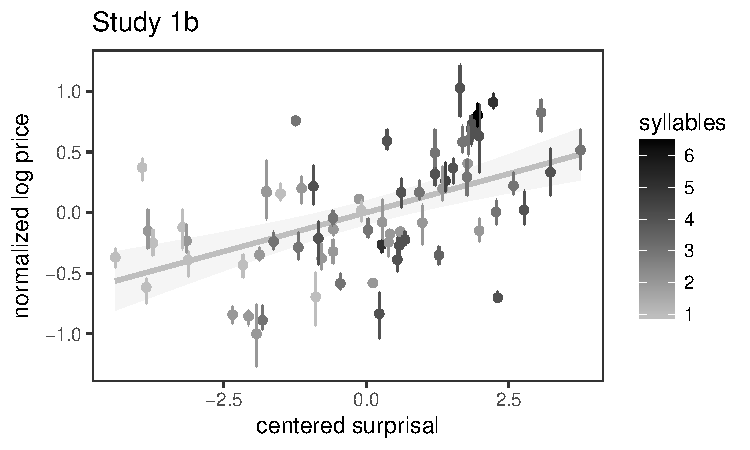
\includegraphics[width=0.5\textwidth]{images/plot_study1b.pdf}
\end{center}
\caption{Results of Study \hyperref[sec:study1b]{1b}. As surprisal and length in syllables increase, participants' scaled free response prices increase.} 
\label{fig:plot_study1b}
\end{figure}

\subsection{Study 2 \label{sec:study2}}

The M-implicature account described above implies that there is no semantic interaction between the intensifier and the adjective it is applied to.
Instead an intensifier should contribute similar cost, and therefore meaning, to the different adjectival phrases in which it occurs\footnote{If the bigram frequency of the modified adjective phrase (\w{very expensive}) deviated from that expected based on independent word frequencies our frequency-based cost account would predict an interactive effect on meaning.
This would likely be a relatively small effect, and the relevant bigrams were too sparse in our corpora to pursue.}.
To explore this issue, we extend our results to additional adjectival scales.
However, most scales are not so easily quantifiable as price; we require a different dependent measure in order to probe them.
For Study \hyperref[sec:study2]{2} we used a forced-ranking dependent measure, which allows us to consider additional adjectival scales.
This dependent measure has the added benefit of providing a more sensitive measure of the differences in degrees between similar adjectival phrases.
This sensitivity also makes Study \hyperref[sec:study2]{2} a better test of the independent effects of length and surprisal.

\subsubsection{Methods}

\paragraph{Participants}

30 participants with US IP addresses were recruited through Amazon's Mechanical Turk and paid \$0.40 for  participation. 2 participants were excluded from the analysis for admitting that they did not think they followed the instructions in a post-experiment survey.

\paragraph{Items}

The full set of intensifiers in Study \hyperref[sec:study2]{2} is identical to that of Study \hyperref[sec:study1a]{1a}. 
%Study \hyperref[sec:study2]{2} is therefore subject to the same systematicity and reproducibility limitations as Study \hyperref[sec:study1a]{1a}, but these concerns are mitigated by the inclusion of our replication Study \hyperref[sec:study1b]{1b}.
For Study \hyperref[sec:study2]{2}, we used a ranking dependent measure: asking participants to sort a set of adjectival phrases according to strength.
Because arranging these phrases required participants to be aware of the full set of adjective phrases and access all of them on the same computer screen (which might vary in size for different participants), not all of our 40 intensifiers could effectively be presented at once.
To make the task easier for participants and to extend to more adjective scales, we divided the full set of intensifiers into 4 smaller sets, maintaining a range of syllable lengths and surprisal across the intensifiers in each smaller set.

With the ranking dependent measure, we no longer need the adjectives to correspond to a standard numeric scale.
We therefore included 4 adjectives: \w{old}, \w{expensive}, \w{beautiful}, and \w{tall}.

\paragraph{Procedure\footnote{A demo of Study \hyperref[sec:study2]{2} can be found at \url{http://cocolab.stanford.edu/links_for_papers/bennett2017extremely/experiments/Study2/.}}}

\begin{figure}[hbt]
\begin{center}
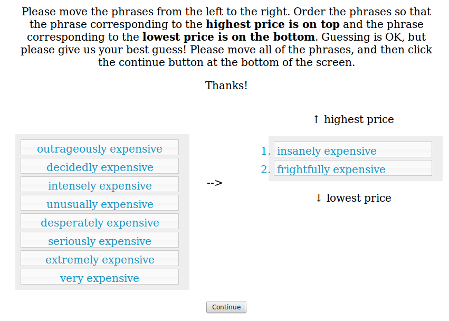
\includegraphics[width=0.4\textwidth]{exp2-q.png}
\end{center}
\caption{Screenshot from Study 2 target question.} 
\label{fig:question_study2}
\end{figure}

For each trial of Study \hyperref[sec:study2]{2}, we asked participants to order a set of 10 adjective phrases according to strength of meaning.
Adjective phrases were randomly ordered in a list on the left.
Participants were asked to move the adjective phrases from the left to the right side of the screen, reordering the phrases from the ``lowest'' to the ``highest'' degree (Figure~\hyperref[fig:question_study2]{\ref{fig:question_study2}}).
Each adjective phrase in a trial contained the same adjective, modified with different intensifiers.
Each participant saw 4 intensifier sets, each paired with one of the four adjectives.
The pairings of intensifier-sets to adjectives varied between participants.
Participants completed 4 such trials, ranking intensifiers for all 4 adjectives and all 4 intensifier sets.

%\begin{table}[ht]
%\begin{center} 
%\footnotesize
%\caption{Intensifier Lists from Experiment 2: Rankings.} 
%\label{exp2-intensifiers} 
%\vskip 0.12in
%%\scalebox{0.3}{
%\begin{tabular}{cccc} 
%\hline
%List A    &  List B & List C & List D \\
%\hline
%surpassingly & colossally & terrifically & frightfully \\
%astoundingly & phenomenally & uncommonly & outrageously \\
%fantastically & mightily & supremely & insanely \\
%strikingly & acutely & awfully & decidedly \\
%excessively & extraordinarily & exceedingly & intensely \\
%markedly & amazingly & radically & unusually \\
%remarkably & terribly & exceptionally & desperately \\
%utterly & notably & incredibly & seriously \\
%truly & significantly & totally & extremely \\
%particularly & quite & especially & very
%\end{tabular}
%%}
%\end{center}
%\end{table}

\subsubsection{Analysis}

We ran a rank-ordered logit model \cite{beggs_assessing_1981, hausman_specifying_1987} with alternative-specific variables for surprisal and for length in syllables. This model did not include an intercept.
%
To test whether we find an interaction between intensifier strength and the adjective it modifies, we ran a second rank-ordered logit model with additional alternative-specific variables for the interaction between the adjective being modified and both surprisal and length. 

\subsubsection{Results}

Our results for Study 2 are shown in Figure~\ref{fig:plot_study2}. In our first model, with surprisal and length as the only predictors in question, we again found a significant effect of surprisal ($b=0.164,t=10.128,p<0.0005$). We also find a significant effect of syllable length ($b=0.243,t=5.888,p<0.0005$).

In likelihood ratio tests, we again found that length alone accounts for the data less well than the full model ($\chi^2(1)=108.085, p<0.0005$) and that surprisal alone also accounts for the data less well than the full model ($\chi^2(1)=34.694, p<0.0005$).
When residualizing length with respect to surprisal, we found a significant effect of surprisal ($b=0.19,t=11.663,p<0.0005$). In addition, with this more sensitive ranking measure, we found a significant effect of length residuals ($b=0.243,t=5.888,p<0.0005$).
When residualizing surprisal with respect to length, we found significant effects of length ($b=0.35,t=8.459,p<0.0005$) and surprisal residuals ($b=0.164,t=10.128,p<0.0005$).

In the second model, with adjective interactions, we again found significant effects of surprisal ($b=0.074, t=2.482, p=0.0131$) and length ($b=0.318, t=3.658, p=0.0003$), and also found a significant interaction between surprisal and the adjective being modified (estimates for \w{tall} and \w{expensive} were higher than for \w{beautiful}, while \w{old} was not significantly different from \w{beautiful}).
This suggests that context-specific surprisal (e.g.~bigram frequencies) might affect the utterance cost, or that factors of utterance cost might have different effects for different adjectives.

In other words, we again found that participants assign stronger interpretations to intensifiers with higher surprisals and/or higher syllable lengths, extending now across four different adjectival scales.
In addition, we found interactions between modifier and adjective (or perhaps scale).

\begin{figure*}[hbt]
\begin{center}
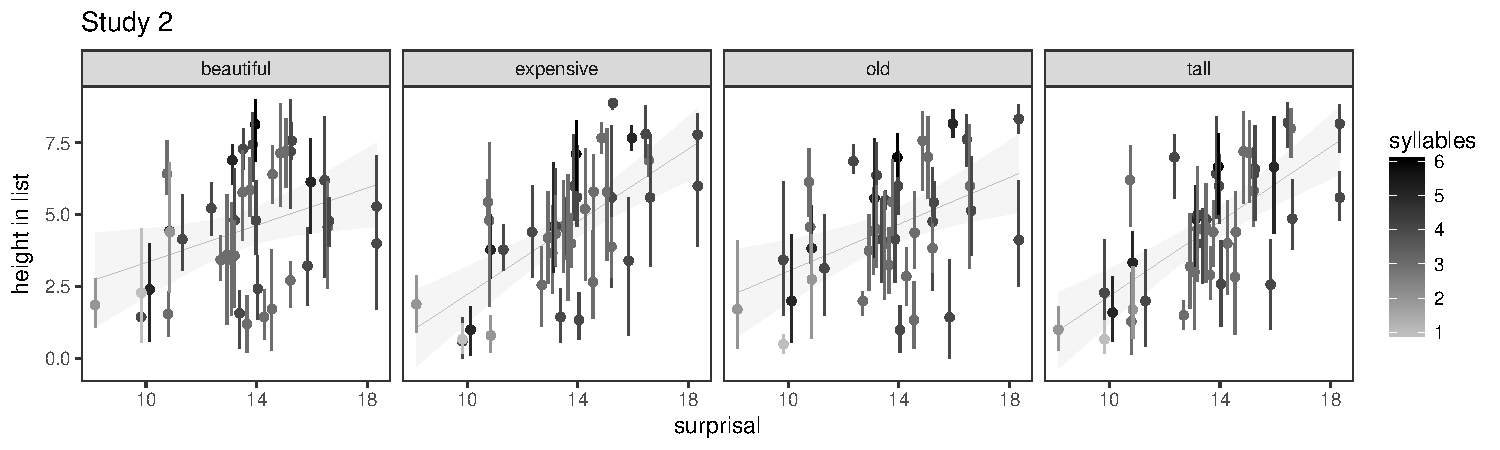
\includegraphics[width=\textwidth]{images/plot_study2.pdf}
\end{center}
\caption{Results of Study 2. As surprisal and length in syllables increase, participants' rankings increased.} 
\label{fig:plot_study2}
\end{figure*}

\subsection{Discussion}

In Studies 1a and 1b, we found evidence that an intensifier's surprisal is a significant predictor of strength of its meaning. In Study 2, we used a more sensitive dependent measure and showed that length in syllables is also a significant predictor of strength of meaning.
These studies taken together provide evidence that intensifier meanings depend systematically on the length and frequency of distribution of their word forms.

While it is unlikely that this accounts for all intensifier meaning, it does suggest that a major portion of meaning comes not from arbitrary, conventional association of signal to sign \cite{de_saussure_nature_1916}, but systematically from features of the word's form and distribution.

Since this is a correlational study, such a relationship does not confirm that an intensifier's cost \emph{causes} it to have a given meaning.

In particular, we can explain the correlation with rarity if the strength of an intensifier's meaning causes it to be rarely used.
That is, more extreme intensifiers naturally refer to less probable events and properties in the world, and therefore might be used less frequently\footnote{
However, note that the frequency with which things occur in the world does not map directly on to how often those things are talked about. 
Although it seems reasonable to suspect that word frequencies reflect the probabilities of the real-world concepts they describe, it might also be the case that improbable things are more likely to be commented on, and so to a certain extent the frequencies of words that describe rare concepts will be inflated. 
}.
Syllable length in turn can depend on the frequency, simplicity, or predictability of a word \cite{zipf_psycho-biology_1935, lewis_conceptual_2016, mahowald_info/information_2013}, either because words that are frequently used get shortened over time \cite{kanwal_evolution_2016} or perhaps because words that refer to simpler or more common concepts enter the lexicon sooner (when more short word forms remain to be assigned meanings).
It is therefore possible that neither of these measures of cost have causal influence on the meanings of intensifiers within a particular communicative act.

To more directly address the question of whether utterance cost \emph{causes} people to interpret an intensifier as stronger, we ran Studies 3 and 4, where we directly manipulated one of our measures of cost---length---in novel intensifiers which have no conventional meaning associated to them. 

\section{Novel intensifier length increases strength of interpretation}

Although the meanings of our existing English intensifiers could have influenced their lengths and frequencies over time, novel intensifiers have no meaning already associated with them. Therefore, if we found a relationship between the length of a novel intensifier and its interpreted meaning, we would have evidence that length can causally influence meaning. In the following two experiments, we directly manipulate the lengths of novel intensifiers and show that longer novel intensifiers are interpreted as having stronger meanings.

\subsection{Study 3 \label{sec:study3}}

%\subsection{Experiment 3\footnote{The full experiment can be found at \url{http://cocolab.stanford.edu/cogsci2015/intensifiers/Experiment3}}}

In Study~\hyperref[sec:study3]{3} we show that longer novel intensifiers are interpreted as having stronger meanings, using our dependent measure from Study~\hyperref[sec:study1a]{1a}.

\subsubsection{Method}

\paragraph{Participants}

30 participants with US IP addresses were recruited through Amazon's Mechanical Turk and paid \$0.80 for their participation. 2 participants were excluded from the analysis for admitting that they did not think they followed the instructions in a post-expeirment survey and 1 for being a non-native Enlgish speaker.

\paragraph{Items}

In Study \hyperref[sec:study1a]{1a}, we rescaled prices within participants and objects.
In order to do the same normalization for novel intensifiers, we chose 9 filler intensifiers to include in Study~\hyperref[sec:study3]{3}.
We chose a set of filler intensifiers to cover a wide range of surprisals and syllable lengths: \w{colossally}, \w{phenomenally}, \w{mightily}, \w{extraordinarily}, \w{amazingly}, \w{terribly}, \w{notably}, \w{significantly}, \w{quite}.
Other than covering a range of prices, the particular choice of fillers should not affect our analysis of the novel intensifiers.
Each novel intensifier was presented in the same context of 9 filler intensifiers.
Eliciting ratings for existing English intensifiers along with novel intensifiers allowed us to again rescale and normalize responses within participants and items, placing all responses for the novel intensifiers on the same scale.
It also allowed us to somewhat obscure our use of fabricated words, and thus decrease task demand.

We varied the novel intensifier between participants from a set of 6 novel intensifiers, three of which were relatively short (\w{lopusly}, \w{ratumly}, and \w{bugornly}) and three of which shared the same ``root'' but were two CVCV syllables longer (\w{fepolopusly}, \w{gaburatumly}, and \w{tupabugornly}).
These items were taken from in previous studies on complexity bias \cite{lewis_conceptual_2016} and modified by adding a final \w{-ly} suffix.

\paragraph{Procedure\footnote{A demo of Study \hyperref[sec:study3]{3} can be found at \url{http://cocolab.stanford.edu/links_for_papers/bennett2017extremely/experiments/Study3/.}}}

The procedure for Study~\hyperref[sec:study3]{3} was identical to that of Study \hyperref[sec:study1a]{1a}, except that we included only a subset of the intensifiers from Study \hyperref[sec:study1a]{1a} and each participant also saw one novel intensifier, randomly mixed in with the rest.

Participants again estimated prices for objects of three different categories paired with all of the intensifiers.
The order of the questions was randomized between and within participants.

\subsubsection{Analysis}

In Study 3,  to study the effect of the length of a novel intensifier on its interpretation, we ran a linear mixed effects model on only the novel intensifiers, with length (``long''=1 or ``short''=-1) as a fixed effect, a random slope for participant, and random intercepts for the three different ``roots''.

We included as filler a subset of the intensifiers we tested in Study 1a, and so we also confirmed our findings from Study 1a.
As in Study 1a, we ran a linear mixed effects regression with centered fixed effects of length and surprisal and a random slope for participant.
%, and a random intercept for intensifier.
%
To see the effect of the two measures of communicative cost separately, we compared the full model to a model without that measure as a regressor using a likelihood ratio test and ran versions of the model where we first residualized the measures with respect to one another.

\begin{figure}[hbt]
\begin{center}
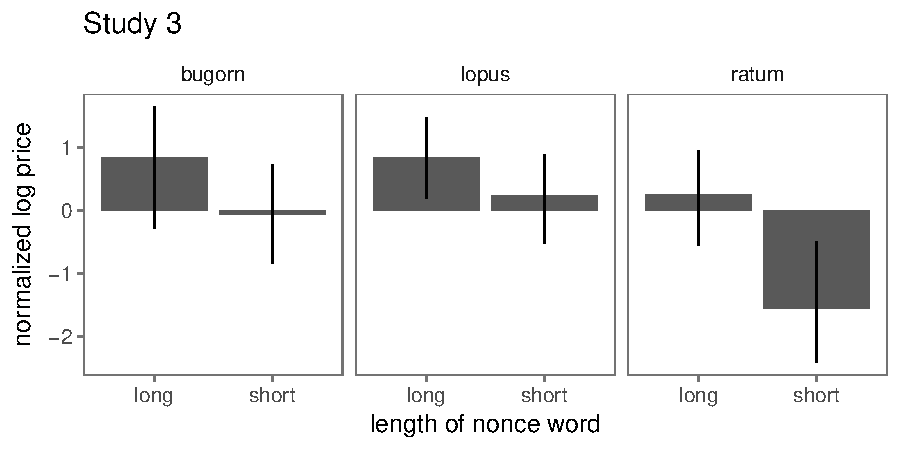
\includegraphics[width=.5\textwidth]{images/plot_study3_A.pdf}
\end{center}
\caption{In Study 3, we found a significant effect of length for all novel intensifiers.} 
\label{fig:plot_study3_barplot}
\end{figure}

\begin{figure}[hbt]
\begin{center}
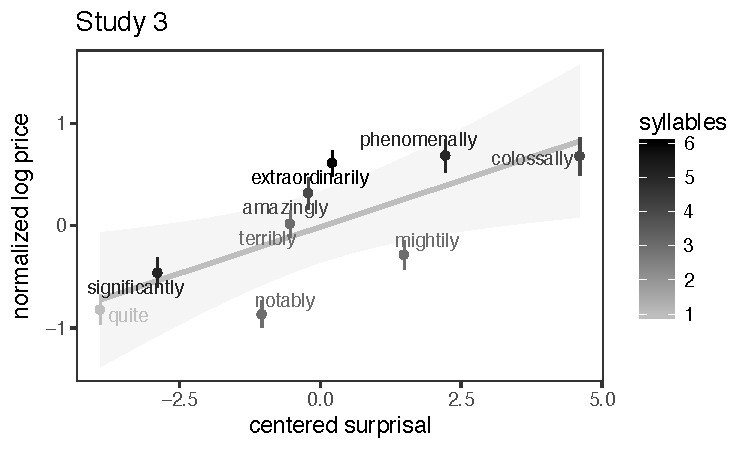
\includegraphics[width=0.5\textwidth]{images/plot_study3_B.pdf}
\end{center}
\caption{In Study 3, we replicated our findings from Study 1a.}
\label{fig:plot_study3_scatter}
\end{figure}

\subsubsection{Results}

In our analysis of novel intensifiers, we found a significant effect of length condition ($b=0.538$, $SE=0.195$, $t=2.757$, $p<0.05$), indicating that people a longer intensifier as stronger, even for novel intensifiers with no conventional meaning (Figure \ref{fig:plot_study3_barplot}).

Replicating our findings from Study 1a, we found significant main effects of surprisal ($b=0.14,t(7.2)=2.49,p=0.0407$) but no significant effect of syllable length ($b=0.194,t(6.3)=2.046,p=0.0846$) (Figure \ref{fig:plot_study3_scatter}). In likelihood ratio test, we found that the full model was a better fit than the model with surprisal only ($\chi^2(8)=8.296,p=0.0403$) and the model with length only ($\chi^2(8)=39.194,p<0.0005$). Residualizing each regressor with respect to one another, we again found qualitatively similar effects to Studies 1a and 1b.

%report(m_resid_syll, "surprisal.centered")
%[1] "$b=0.182, t(26)=9.495, p<0.0005$"
%> report(m_resid_syll, "syll_resid")
%[1] "$b=0.194, t(26)=8.268, p<0.0005$"
%> report(m_resid_surp, "surprisal_resid")
%[1] "$b=0.14, t(26)=7.094, p<0.0005$"
%> report(m_resid_surp, "syll.centered")
%[1] "$b=0.286, t(26)=11.952, p<0.0005$"

In a post-hoc regression with a fixed effect for novel adverb root, we found a significant effect of root on response ($F(2)=3.386, p<0.05$), suggesting possible additional effects of form that we have not captured with length in syllables alone.
Average responses for \w{ratumly} were lowest out of all the intensifiers used in Experiment 3, and average responses for \w{tupabugornly} were highest.
The rest of the novel intensifiers had average ratings within the range of the attested intensifiers.

% \todo{discuss novel vs. attested: e.g. what's the inferred surprisal?}

\subsection{Study 4 \label{sec:study4}}

In Study~\hyperref[sec:study4]{4} we again show that longer novel intensifiers are interpreted as having stronger meanings, this time for an additional adjective, using our dependent measure from Study~\hyperref[sec:study2]{2}.

\subsubsection{Methods}

\paragraph{Participants}
60 participants with US IP addresses were recruited through Amazon's Mechanical Turk and paid \$0.16 for their participation. 3 participants were excluded from the analysis for admitting that they did not think they followed the instructions in a post-experiment survey.

\paragraph{Items}

In Study \hyperref[sec:study4]{4}, each participant saw exactly one of two adjectives (\w{expensive} or \w{tall}, varied between participants) with the set of intensifiers from Study \hyperref[sec:study3]{3}. This set included 9 context/filler words and one novel intensifier, which we varied between participants.

\paragraph{Procedure\footnote{A demo of Study \hyperref[sec:study4]{4} can be found at \url{http://cocolab.stanford.edu/links_for_papers/bennett2017extremely/experiments/Study4/.}}}

Except for the the narrower set of items, noted above, Study \hyperref[sec:study4]{4} was identical to Study \hyperref[sec:study2]{2}. 

As in Study \hyperref[sec:study2]{2}, adjective phrases for each intensifier-adjective pairing were initialized on the left in a random order.

\subsubsection{Analysis}

For the novel intensifiers, we ran a cumulative logit model on the rankings (relative to the filler intensifiers) that participants gave to the novel intensifier.

As in Study 2, we also ran such a model with the word stem (or "root") as another regressor.

With our filler intensifiers for Study 4 we again ran a ranked order logit model (re-ranking to ignore novel intensifiers) to confirm effects of syllable length and surprisal.

\subsubsection{Results}

In the cumulative logit model, we found a significant effect of length condition ($b(\mbox{``short''})=-1.41, z=-2.79, p=0.005$).

When we included a regressor for the root of the novel intensifier, we did not find a significant effect of root on participants' relative rankings (for root \w{lopus}, $p=0.110$; for root \w{ratum} $p=0.304$).

Rankings for novel intensifiers had much higher variance than rankings for attested intensifiers, since we had many fewer rankings for the novel intensifiers (which varied between participants) than for the attested ones (which every participant saw once). The novel intensifier \w{ratumly} was again on average ranked as less strong than any other intensifier, but the highest-ranked novel intensifiers (\w{gaburatumly} and \w{tupabugornly}) were on average ranked below the highest-ranked attested intensifiers (\w{colossally}, \w{phenomenally}, \w{extraordinarily}, and \w{amazingly}).

For the filler items, we replicated our findings from Study 2, showing significant effects of both surprisal ($b=0.447,t=13.879,p<0.0005$)
and syllable length ($b=0.581,t=10.738,p<0.0005$) on the order in the list that participants chose for the intensifiers (see Figure \ref{fig:plot_study4}).
Likelihood ratio tests showed significant improvement when including each regressor, and residualized predictors were also significant as in Study 2.
This replication is perhaps unsurprisaing, since we chose intensifiers to cover the full range of surprisal and syllable lengths.

\begin{figure}[hbt]
\begin{center}
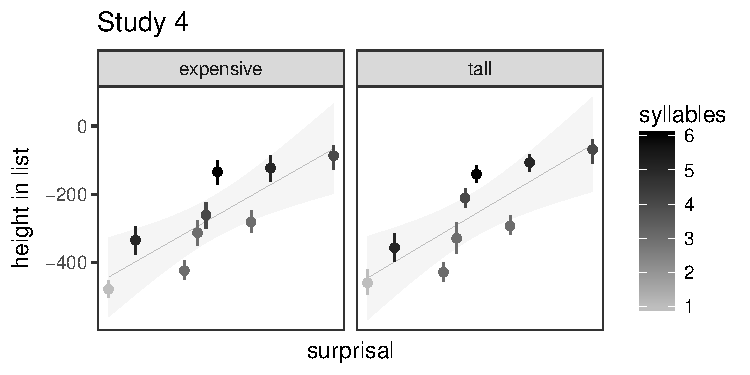
\includegraphics[width=0.5\textwidth]{images/plot_study4.pdf}
\end{center}
\caption{In Study 4, we replicated our finding from Experiment 2: longer and less frequent intensifiers are ranked higher than shorter and more frequent ones.}
\label{fig:plot_study4}
\end{figure}

% \end{figure}

\subsection{Discussion}
Overall, in Studies 3 and 4 we found that word length in syllables is a significant predictor of interpretation strength for novel intensifiers.
These novel intensifiers have no established meaning, so the relationship between their length and strength cannot be a direct consequence of the lexicon becoming more efficient over time.
This result is consistent with the hypothesis that participants are inferring the meanings of the novel intensifiers pragmatically, as in the M-implicature account sketched above.

Alternatively, it could be that participants have learned a general relationship between length and meaning of intensifiers in English, and are utilizing this meta-linguistic knowledge to interpret the new words they encounter.

This meta-linguistic hypothesis is less parsimonious than the pragmatic hypothesis, since the pragmatic hypothesis relies only on mechanisms (M-implicature) that we know to be involved in other examples of language understanding (e.g. as in the ``I got the car to start'' example above).
It builds on previous formal models of adjective meaning and informal models of intensifier meaning, generalizing to a wide range of intensifiers.

Whether due to a process of M-implicature or meta-linguistic knowledge, these results demonstrate that the relationship between word cost and meaning is not merely a static, gradual result of language evolution---interpreted meaning of intensifiers depends on length in an active, dynamic way.

\section{General Discussion}

Motivated by a recent probabilistic model of scalar adjectives \cite{lassiter_context_2013}, we argued that adjectival intensifiers could gain aspects of their meaning through a systematic pragmatic inference, even in the absence of conventional literal meaning.
Our model predicted a linear relationship between the intensity of an intensifier and its communicative cost, measured here in terms of length and negative log-frequency.

In five experiments we provided evidence that intensifier meanings do depend systematically on the length and frequency of occurance of those word forms and that this relationship holds even for novel words.

While it is unlikely that this accounts for all intensifier meaning, it does suggest that a major portion of meaning comes not from arbitrary, conventional association of signal to sign \cite{de_saussure_nature_1916}, but from features of the word's form and distribution, together with inferential processes of listeners.

For the semantics of adverbial modifiers, we have shown how pragmatic mechanisms could be central in establishing flexible contributions to sentence meaning.
We have extended previous proposals that degree adverbs transform or create new threshold variables, providing a concrete mechanism for interpreting an arbitrary degree adverb in an arbitrary context.

This mechanism for linking a parsimonious semantics to interpretation via pragmatic inference follows naturally and straightforwardly from an understanding of rational social agents engaging in communication.
With the minimal assumption that each use of a scalar adjective has a different threshold, we have been able to extend a model of adjective interpretation to account for a major source of intensifier meaning.
This model adds to an abundance of linguistic phenomena --- e.g. aspects of metaphor \cite{kao_formalizing_2014}, prosody \cite{bergen_strategic_2015}, politeness \cite{yoon_i_2017}, and presupposition projection \cite{qing_rational_2016} --- which can be explained within the basic RSA framework, each with minimal, compatible assumptions.
The precise specification of this model is laid out in more detail in the Appendix.

Our proposal and our experiments suggest that even a very minimal semantics for intensifying degree adverbs can be plausible and productive.
We have implemented and described one version of such a semantics, but other versions might exist with different methods of generating the threshold variable for an adjective phrase.

The intensifiers we have looked at may also have other source(s) of meaning in addition to the measures of communicative cost that we have explored.
There appears to be consistent variation in intensifier meaning beyond that explained by our measures of communicative cost.
% \todo{what is a good measure of this? falls under the "variance explained" question}
%\ndg{maybe so how much?}
This may be because we have not exhausted the sources of communicative cost.
It could also be that in addition to the relationship we have described between communicative cost and strength, conventional contributions to meaning are associated with certain adverbs.
 In particular, many intensifiers seem to be derived from adverbs having to do with emotion, and the valence and/or arousal of these root emotions might influence the strength of an intensifier or its affinity to co-occur with some adjective types rather than others.
This might be especially true for intensifiers that are still making the change from manner adverb to intensifier (e.g. terribly once only carried the qualitative meaning of ``bad and frightening'', but now almost exclusively means simply ``a lot'').

%While we have shown, through our use of novel intensifiers, that people can use communicative cost for in-the-moment interpretation, they may not have to.
%It is possible that over time such an interpretation could become lexicalized, become part of the context-independent semantics of that word. \ndg{do we need this par?}

In investigating our proposal proposal of how intensifiers get their meanings, we have collected many judgements about the relative strengths of intensifiers across several adjective scales and dependent measures.
As a summary of these judgements, we have aggregated across the different dependent measures in our studies and displayed them in a common scale in Figure~\ref{fig:intensities}.
For each study, we computed the average value of the dependent measure (normalized log-transformed price for Studies 1a, 1b and 3 and height in list for Studies 2 and 4) for each intensifier in that study. We then z-scored within the study, so that our different operationalizations of ``strength'' in the different study designs could be reasonably compared together.
Given this rescaling, we can compare the strengths of these intensifiers to one another, including the novel intensifiers from Studies 3 and 4.
%\ndg{say something about what we see here?}
We see some consistency across experiments and show that our choices of novel intensifiers spanned the full range of natural intensifier strengths.

For the broader question of form-meaning mapping, we have suggested a source of non-arbitrary association based on both properties of the word form and of its distribution.
The effect of a word's distribution on its interpretation has potentially interesting implications for language change.
If the distribution of a particular grammatical category of word (e.g. intensifiers) influences its meaning and the meaning of a word in turn influences its distribution, this would result in an unstable lexicon for this grammatical category.
This suggests a mechanism by which overused words might become stale, and would predict the rapid creation of new, unusual intensifiers.
This process indeed seems to be evident in the history of English \cite{bolinger_degree_1972}.
% While we have described some evidence for this distributional source of meaning, further work will be necessary to separate the influence of the form of a word from the influence of its distribution.
%A fuller understanding of these factors would also enable us to explore word-types that support a similar relationships between distribution and meaning.

We have argued that form-to-meaning mapping can come about through the inferences known to support pragmatic interpretation.
Seen another way, the basic assumption that people are actively trying to communicate with each other---each reasoning about what the interlocutor means---\emph{requires} non-arbitrary relationships between a variety of factors and effective meaning.
Some systematic aspects of meaning follow directly from the principles of language understanding.

%\todo[inline]{if room could say something about next steps. also relation to other's work on meaning.}

\begin{figure}[hbt]
\begin{center}
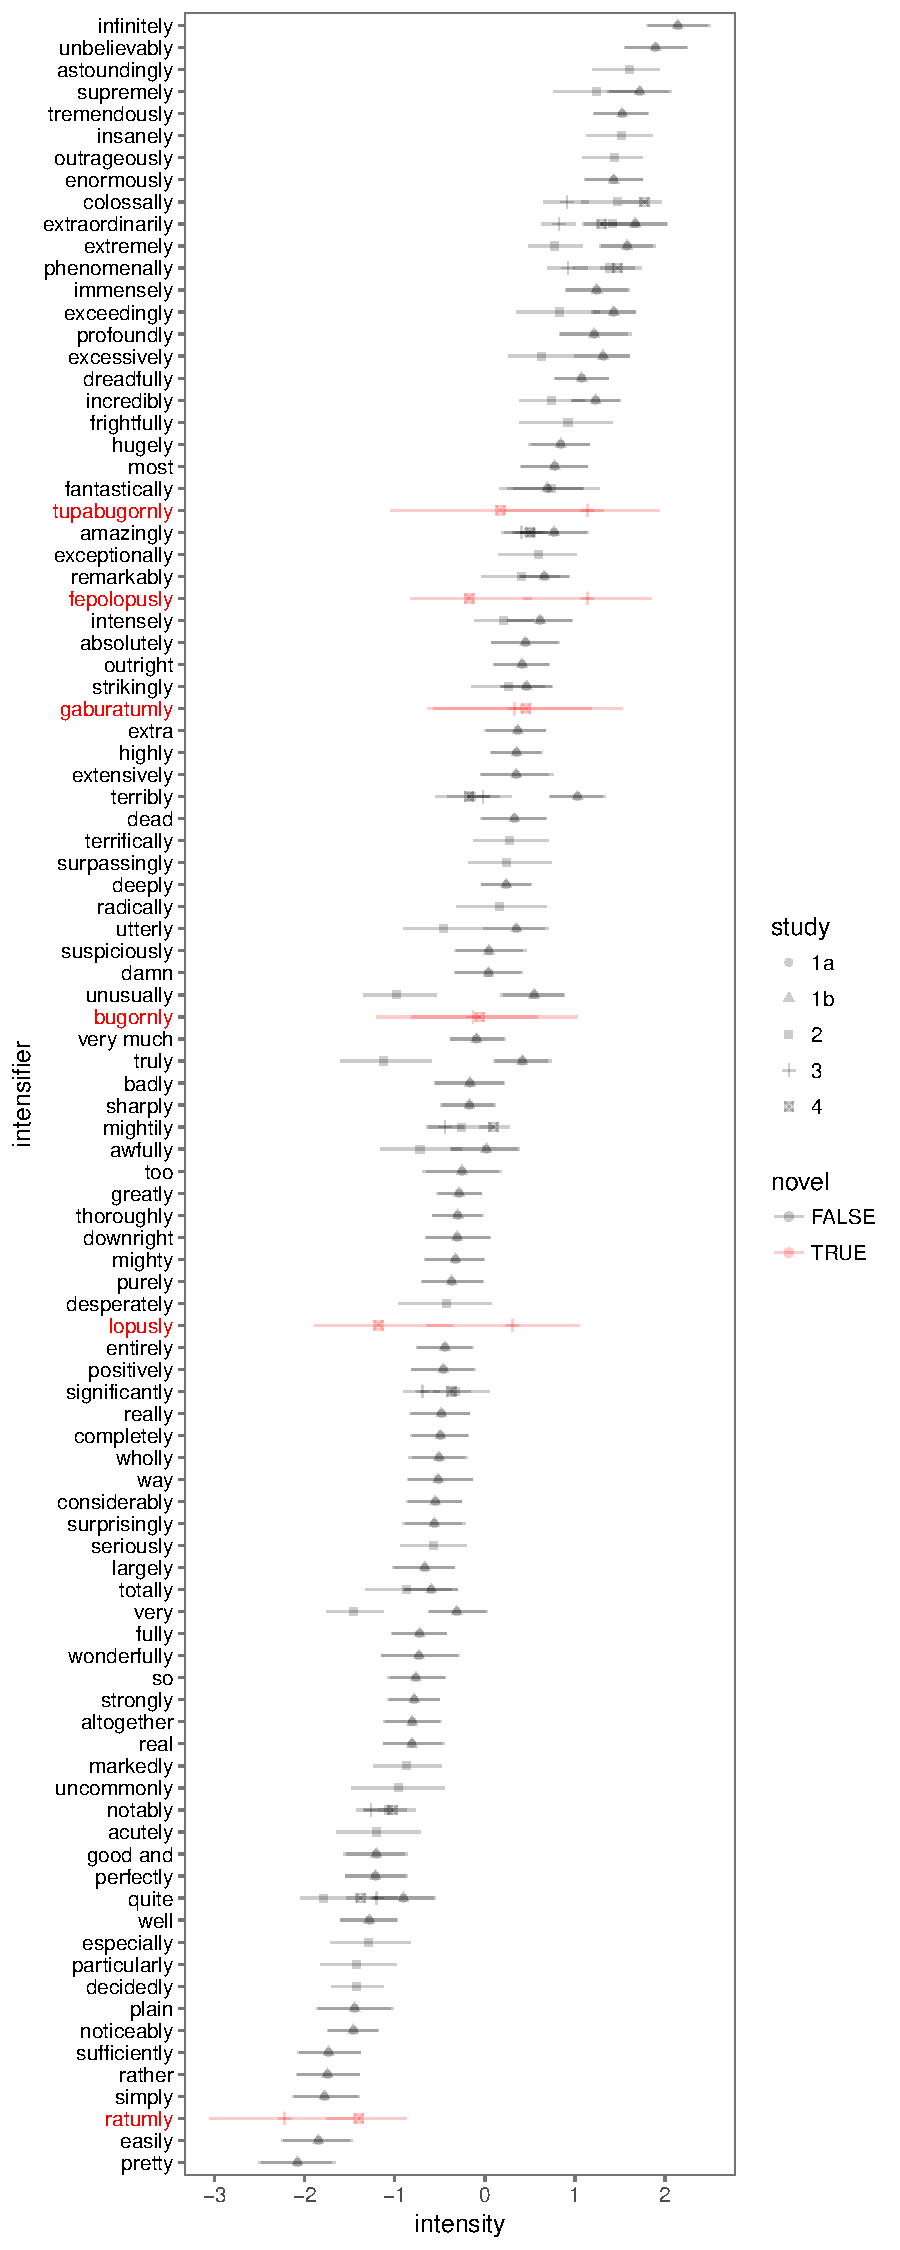
\includegraphics[width=0.5\textwidth]{images/intensities.pdf}
\end{center}
\caption{Intensities (each dependent measure, z-scored) of all intensifiers across all 5 studies. Novel intensifiers are shown in red, standard English intensifiers in black.}
\label{fig:intensities}
\end{figure}

\section{Acknowledgments}

This work was supported by a James S. McDonnell Foundation Scholar Award to NDG and ONR grant N00014-13-1-0788.

\bibliographystyle{apacite}

\setlength{\bibleftmargin}{.125in}
\setlength{\bibindent}{-\bibleftmargin}

\bibliography{intensifiers}

\section{Appendix} \label{app:model}

 \citeA{lassiter_context_2013}'s model of scalar adjectives belongs to the family of Rational Speech Act (RSA) models in which speaker and listener communicate by  reasoning about each other's goals and inferences (\citeNP{frank_predicting_2012, goodman_knowledge_2013}; for related models, see also \citeNP{franke_quantity_2011, russell_probabilistic_2012}). 
 These models have been shown to account for a number of key phenomena in pragmatics. The adjective model accounts for uncertainty about the adjectival threshold by including a semantic variable, which the pragmatic listener infers at the same time that she infers the speaker's intended meaning. 

RSA models begin with a literal listener, which captures the semantic denotation of sentences. 
We assume adjectival phrases with the same scale and polarity have the same denotation. For example, \w{expensive}, \w{very expensive} and \w{phenomenally expensive} all denote: $\lambda x . \text{price}(x) > \theta_i$. %unpack?
However, every adjective phrase has its own threshold variable $\theta_i$,\footnote{Other versions of this model could easily be imagined in which the threshold for an adjective phrase is determined by the basic threshold for the adjective and some transformation on that threshold (e.g. multiplication, addition, etc.) caused by the intensifier. If the transformation is mostly regular, with a single parameter needing to be inferred for each intensifier, and if the values of these parameters are inferred for each adjective phrase, then such a model would be functionally equivalent to the one we describe here.} together notated $\vec{\theta}$, allowing their meanings to differ.
Given an utterance $u_i$ (e.g. an \w{expensive laptop} or a \w{very expensive laptop}) and a set of thresholds, a literal listener $L_0$ will use Bayesian inference to update his prior beliefs $P(d)$ about the degree $d$ (e.g. the laptop's price) given that the degree is greater than the threshold for that utterance.

$$P_{L_0}(d|u_i, \theta_i) \propto P(d) \cdot \delta_{d > \theta_i}$$

A speaker with the goal of communicating some actual degree $d$ assigns a utility $\mathbb{U}(u_i|d)$ to each utterance such that he prefers utterances which will inform the literal listener, but avoids utterance cost, $C(u_i)$:

$$\mathbb{U}(u_i | d, \vec{\theta}) =  \ln\left(P_{L_0}(d | u_i, \theta_i) \right) - C(u_i) $$

Given a set of alternative utterances (e.g. the speaker might be choosing between saying \w{very expensive} as opposed to \w{expensive} or \w{extremely expensive}, or saying nothing at all), the speaker $S_1$ will choose utterances according to a softmax decision rule \cite{sutton} with optimality parameter $\lambda$, so that:

$$ P_{S_1}(u_i | d, \vec{\theta}) \propto e^{\lambda \mathbb{U}(u_i | d, \vec{\theta})} $$

A pragmatic listener $L_1$ uses the prior probability, $P(d)$, of different degrees, along with knowledge of the cost of each utterance, in order to guess both the thresholds for each utterance and which degree the speaker intended to communicate\footnote{We assume a uniform prior on thresholds $\theta_i$.}:

$$ P_{L_1}(d, \vec{\theta} | u_i) \propto P(d) \cdot P_{S_1}(u_i | d, \vec{\theta}) $$

We simulated such a model with three alternative adjective phrases (i.e.~three intensifiers) with costs of $1$, $5$, and $10$. We also included a null utterance, with trivial meaning (always true) and cost of $0$. The prior distribution of degrees along this adjective's scale (which we will discuss as ``prices'' for concreteness and consistency with our Experiment 1) was a gaussian peaked at $0$.
We used an optimality parameter of $\lambda=5$ in our simulation. 

Though the literal semantics are identical (but permitting different threshold parameters), the different phrases received different interpretations: the more costly intensifiers corresponded to less probable, more extreme prices (Figure ~\ref{model}).
This can be seen as an M-implicature: more costly intensifiers are assigned stronger, less probable, meanings. 
The model therefore predicts an association between intensifier meaning and utterance cost (see \citeA{bergen_pragmatic_2014} for other M-implicature models within the RSA framework).

\begin{figure}[tbh]
\begin{center}
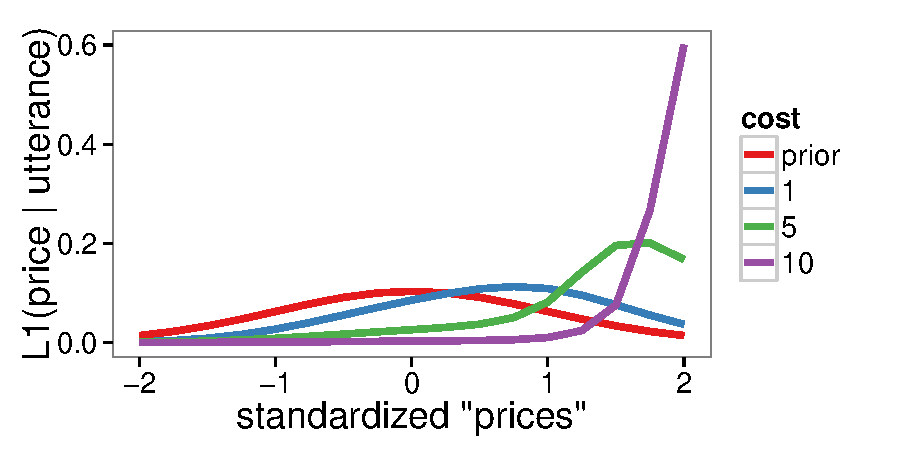
\includegraphics[width=0.4\textwidth]{model_results.pdf}
\end{center}
\caption{Modeling intensifiers as M-implicature: more costly intensifiers correspond to more extreme meanings.} 
\label{model}
\end{figure}

Top assess the quantitative relationship between cost and meaning, we ran a second simulation, identical as the first except using 6 different utterance costs (or ``intensifiers'').
The quantitative form predicted by the model is a approximately linear (Figure \ref{model-heights}).
It is this simple prediction that we test in the main text.

\begin{figure}[tbh]
\begin{center}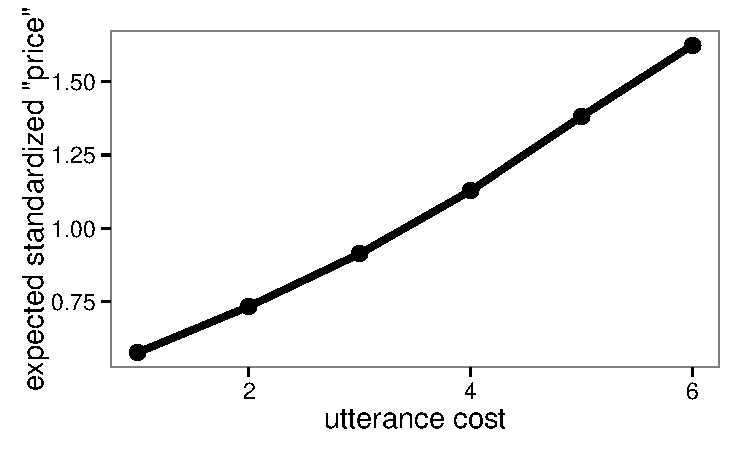
\includegraphics[width=0.4\textwidth]{height-by-cost.pdf}
\end{center}
\caption{Model prediction of expected price as cost of intensifier increases, based on intensifiers evenly spaced in cost. The relationship is approximately linear.} 
\label{model-heights}
\end{figure}

\end{document}
